\documentclass{llncs}

\usepackage{hyperref}
\hypersetup{
    colorlinks,
    citecolor=black,
    filecolor=black,
    linkcolor=black,
    urlcolor=black
}
\usepackage{makeidx}  
\usepackage{amsmath}
\usepackage{amsfonts}
\usepackage{amssymb}
\usepackage{listings}
\usepackage{graphicx}
\usepackage[rightcaption]{sidecap}
\setcounter{tocdepth}{2}
\usepackage{hyperref}
\usepackage{pythonhighlight}

\begin{document}

         % for the preliminaries
%
\title{Diseño, implementación, evaluación y añálisis de un Sistema de Recuperación de Información para recuperar documentos PDF y txt}
\author{David Orlando De Quesada Oliva, Javier Dom\'inguez}
\institute{MATCOM, Universidad de La Habana.\\
\email{d.quesada@estudiantes.matcom.uh.cu, j.dominguez@estudiantes.matcom.uh.cu}\\
\texttt{}
}
\maketitle

\begin{abstract}
    
    Este art\'iculo aborda sobre la implementación de un Sistema de Recuperación de Información para la recuperación 
    de documentos de texto en distintos formatos. Se aborda los distintos pasos para el preprocesamiento del texto 
    y las consultas, la realización y explicación de los modelos usados, la evaluación usando el modelo principal 
    y la presentanción de una interfaz de usuario para la realización de las consultas.
    
   \keywords{pdf, txt, idf, tf, peso, nltk, fuzzy, vectorial, preprocesado, peso}
\end{abstract}

\tableofcontents
%

% start of the contributions


\chapter*{Herramientas empleadas en el desarrollo del sistema}
\addcontentsline{toc}{chapter}{Herramientas usadas para el el desarrollo del sistema}

Para el desarrollo del sistema usamos Python como lenguaje de programación.\\ 
Librerías de Python que utilizamos:\\

\noindent $\bullet$ nltk, para los stopwords, stemming y lemmatizing. \\
$\bullet$ streamlit para la interfaz gráfica. \\
$\bullet$ pdfminer y fpdf para procesar archivos .pdf.\\
$\bullet$ inflect para convertir números a sus representaciones textuales\\
$\bullet$ streamlit para la interfaz gráfica \\
$\bullet$ pandas para trabajar con dataframe \\\\
Para correr la aplicación escriba en consola: \\\\
\begin{python}
    streamlit run main.py
\end{python}


% \newpage
\chapter*{Proceso para la creación de un sistema de recuperación de información de documentos}
\addcontentsline{toc}{chapter}{Proceso para la creación de un sistema de recuperación de información de documentos}

\section{Preprocesamiento del texto:}

Siempre que tengamos datos textuales, debemos aplicar varios pasos de preprocesamiento a los 
datos para transformar palabras en tokens que permitan un mejor resultado del modelo.
En el sistema de recuperación de información que se implementó es posible aplicar 
los siguientes pasos de preprocesamiento del texto. La implementación de los mismo está en 
el file \textbf{text processing.py}. En muchos pasos hacemos uso de la librería NLTK (Natural Language Toolkit)
de Python.
\\

\noindent
\textbf{Llevar el texto a minúsculas:}
Se lleva todo el texto a minúsculas para reducir el tama\~{n}o del vocabulario de nuestro texto.

\noindent
\textbf{Implementación hecha en Python:}
\begin{python}
    def text_to_lowercase(text: str):
        return text.lower()
\end{python}

\noindent
\textbf{Remover números:}\\
Podemos remover los números o convertir los números en sus representaciones textuales. 

\noindent
\textbf{Implementación hecha en Python haciendo uso de expresiones regulares para eliminar los números:}
\begin{python}
    import re
    def remove_numbers(text):
        return re.sub(r'\d+', '', text)
\end{python}

\noindent
\textbf{Implementación hecha en Python parar convertir los números a sus expresiones textuales haciendo uso de la libería inflect:}
\begin{python}
    import inflect
    def convert_numbers_into_words(text: str)-> str:
        result = []
        for word in text.split(): 
            if word.isdigit(): 
                result.append((inflect_engine.number_to_words(word)))
            else:
                result.append(word)

        return ' '.join(result)
\end{python}


\noindent
\textbf{Remover los signos de puntuación:}\\ 
\noindent
Eliminamos los signos de puntuación para no tener diferentes formas de la misma palabra. 
Si no eliminamos los signos de puntuación, entonces  por ejemplo \textbf{call.} \textbf{call!} 
\textbf{,call}  serán tratados por separado cuando deberían referirse a la misma palabra.
\\
\textbf{Implementación hecha en Python parar remover los signos de puntuación:}
\begin{python}
    def remove_punctuation_marks(text: str):
        translator = str.maketrans('', '', string.punctuation)
        return text.translate(translator)
\end{python}

\noindent
\textbf{Remover los stopwords:}\\ 
\noindent
Los stopwords son palabras que no contribuyen al significado de una oración. Por tanto
pueden eliminarse con seguridad sin causar algún cambio en el significado de la oración.
La biblioteca NLTK tiene un conjunto de stopwords y podemos usarlas para eliminar 
los stopwords de nuestro texto y devolver una lista de tokens de palabras. 

\begin{SCfigure}[0.6]
    \caption{Lista de stopwords de NLTK}
    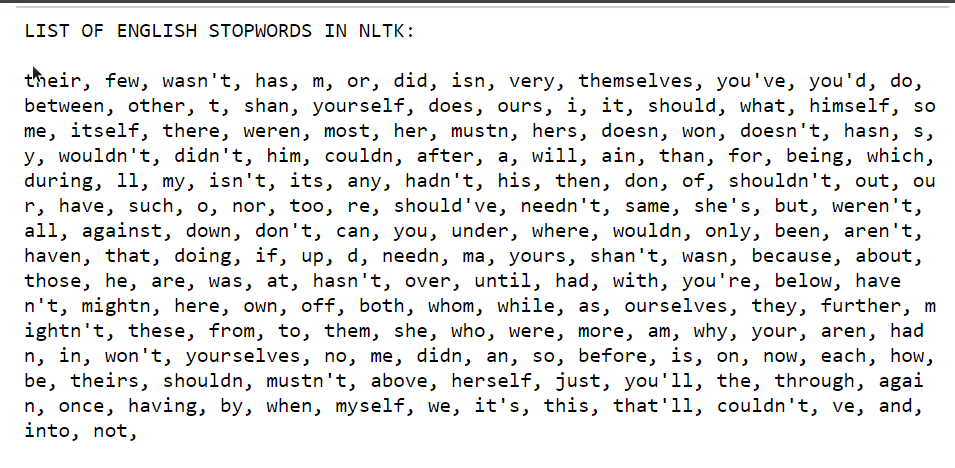
\includegraphics[scale = .3]{./images/englis_stopwords_nltk.png}
\end{SCfigure}

\noindent
\textbf{Implementación hecha en Python para el proceso de eliminar los stopwords}

\begin{python}
    from nltk.corpus import stopwords
    def text_remove_stopword(text: str):
        stop_words = set(stopwords.words("english"))  
        return ' '.join([word for word in text_tokenize(text) if word not in stop_words])
    
\end{python}

\noindent
\textbf{Stemming:}\\ 
\noindent
El stemming es el proceso mediante el cual se obtiene la raíz gramatical de una palabra. 
Stem es la parte a la que se le añaden los afijos flexivos (-ed, -ize, -de, -s, etc. En el caso del idioma inglés)
El stem de una palabra es creado removiendo el prefijo o sufijo de la palabra. Por lo que el proceso
de stemming de una palabra puede no resultar en palabras gramaticalmentes correctas del idioma

\begin{SCfigure}[0.6]
    
    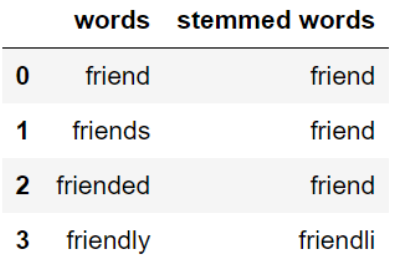
\includegraphics[scale = .3]{./images/stemming1png.png}
    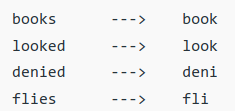
\includegraphics[scale = .7]{./images/stemming2png.png}
    \caption{Ejemplos del proceso de stemming en algunas palabras}
\end{SCfigure}

Hay principalmente 3 algoritmos para hacer stemming \textbf{Porter Stemming}, 
\textbf{ Snowball Stemmer} y el \textbf{Lancaster Stemmer}. El Porter Stemming 
es el más usado entre ellos.
\\\\
\textbf{Implementación hecha en Python para hacer el proceso de stemming. Se puede pasar como parámetro un string que indica con cual de los tres algoritmos se quiere hacer stemming.}

\begin{python}
    from nltk.stem.porter import PorterStemmer
    from nltk.stem.snowball import SnowballStemmer
    from nltk.stem.lancaster import LancasterStemmer

    porter_stemmer =  PorterStemmer()
    snowball_stemmer = SnowballStemmer(language='english')
    lancaster_stemmer = LancasterStemmer()
\end{python}


\begin{python}
    def text_stem_words(text: str, stemmer: str):
        if text == 'porter':
            stemmer = porter_stemmer
        elif text == 'snowball':
            stemmer = snowball_stemmer
        else:
            stemmer = lancaster_stemmer

        stems = [stemmer.stem(word) for word in text_tokenize(text)]
        return ' '.join(stems)
\end{python}

\noindent
\textbf{Lemmatizing:}\\
Como el stemming, el proceso de lemmatizing también convierte una palabra
a su raíz gramatical. La única diferencia es que el lemmatizing asegura que
la raíz gramatical de la palabra pertenezca al lenguaje. Obtenemos palabras
válidas si usamos el lemmatizing. En \textbf{NLTK}, podemos hacer uso del 
\textbf{WordNetLemmatizer} para obtener los lemmas de las palabras. 

\noindent
\textbf{Implementación en Python para el proceso de lemmatizing usando el WordNet de NLTK}

\begin{python}
from nltk.stem import WordNetLemmatizer
lemmatizer = WordNetLemmatizer()
def text_lemmatize_words(text: str):
lemmas = [lemmatizer.lemmatize(word, pos ='v') for word in text_tokenize(text)]
return ' '.join(lemmas)
\end{python}

\noindent
\textbf{Separar el texto en tokens:}\\
El último paso que hacemos siempre (este paso es necesario) 
es separar el texto en una lista de tokens de palabras 
removiendo los espacios. Para eso hacemos uso del word tokenize 
de NLTK.
\\\\
\noindent
\textbf{Implementación en Python para separar el texto en tokens}

\begin{python}
from nltk.tokenize import word_tokenize
def text_tokenize(text: str):
    tokens = word_tokenize(text)
    return tokens
\end{python}
\noindent
De la forma en que está hecho el código se le puede pasar uno o varios pasos de preprocesamiento 
al texto según se requiera. 
\\
\begin{python}
def text_preprocessing(*, text: str, 
    lowercase: bool = False, 
    remove_numbers: bool = False,
    convert_numbers: bool = False,
    remove_punctuation: bool = False,
    stopwords: bool = False,
    stem: str = None,
    lemmatize: bool = False):
    ...
\end{python}
El método recibe un texto y se le pasan en True los parámetros con los que
se quiere filtrar el mismo. En el caso del parámetro stem se le pasa un string 
que indica con cual de los algoritmos se va a hacer el stemming. 

\noindent
\textbf{Configuración predeterminada empleada:}
\begin{python}
def filter_and_tokenize_text(text: str):
    tokens = text_preprocessing(
                text=text,
                lowercase = True,
                convert_numbers= True,
                remove_punctuation=True,
                stopwords=True,
                lemmatize=True

            )

    return tokens
\end{python}

\noindent
Este preprocesado de texto se le hace tanto a los documentos en el sistema como
a cada query que se procese del usuario.

\section{Tokenización de los documentos del sistema y creación del vocabulario de las palabras:}
Por defecto todos los documentos que tiene el sistem están en el path:
\begin{python}
'.\system_docs'
\end{python}

Para el preprocesado de los documentos del sistema se va por cada file del path y
se lee el texto del documento(la forma de leer varía según el formto del mismo, consideramos
aceptar .txt, pdfs y textos planos sin extensión) contruimos una instancia de Doc con el nombre 
del documento, el path donde está realmente(útil para cuando el usuario haga la búsqueda
pueda descargar el documento original), el tipo (TXT, PDF, o Texto Plano son los que consideramos),
y el texto que al inicializarse se procesa el texto como se explicó  previamente y nos quedamos con una lista 
de tokens que representan las palabras que tienen significación en ese el texto.
\begin{python}
class Doc:

    def __init__(self, name: str, path: str, type: str, text= str):
        self.name = name
        self.path = path
        self.type = type
        self.terms = filter_and_tokenize_text(text)
    ...
\end{python}

Si en el path hay un folder se va recursivo por cada folder y se aplica lo mismo. De esta forma se va
construyendo una lista de Doc que representan la información necesaria de los documemntos que hay en el 
sistema. Al mismo tiempo se construye una lista con todos los términos distintos que aparecen en todos 
los documentos. Hacer estas operaciones son bastante costosas cuando se tienen bastante documentos en 
el sismtema por lo que se hace solo cuando sea necesario porque se cambió o añadió nuevos documentos.
Por lo que una vez obtenido las dos listas se serializa y guarda con \textbf{pickle} en los files 
{documentos.pickel} y \textbf{terms.pickle}. De esta forma no hay que estar generando cada vez sino que
se lee el archivo.

El código de implementación de este proceso está en 
\begin{python}
    system_docs_preprocessing.py
\end{python}

Para decir que se quiere hacer el preprocesado de los documentos del sistema y generar nuevos files 
se llama al handler con el parámetro system docs preprocess required en True
\begin{python}
handler =  Retrieval_handler(system_docs_preprocess_required=True,
     model_preprocess_required=True, retrieval_model_used='vectorial')
    ...
\end{python}

En caso que sea False el handler internamente cargará los files pickle correspondientes.

\section{Tokenización de la query}:
Similar a como se realiza con los documentos existentes en el corpus el texto de una query
se procesa aplicado los filtros visto anteriormente y te quedas al final con la lista 
de tokens que representan las palabras significativas de la mismas.  Los términos 
que esta lista de tokens que no estén en el vocabulario se eliminan de la misma.

\begin{python}
def remove_terms_not_appear(q_terms, terms):
    result = []
    for t in q_terms:
        if t in terms:
            result.append(t)
    return result
...
\end{python}

\section{Aplicación del modelo}
\subsection{Modelo vectorial:}
El modelo principal que usamos para el sistema de recuperación de información fue el vectorial.
Este modelo representa los documentos como vectores en un espacio vectorial común, donde cada 
dimensión corresponde a un término independiente. \\
Por ejemplo: \\
Sea dj el documento j y i,...t el t-ésimo término entonces el vector del documento j quedaría:\\
$
    d_j = (w_{1,j}, w_{2,j}, ..., w_{t,j})
$

\noindent
Si aparece un término en el documento, su valor 
en el vector es distinto de 0. El esquema usado para calcular estos valores se conoce como
\textbf{tf-idf weighting}. El peso(weight) asociado al par $(t_i, d_j)$ es $>=0$. 
\\\\
\noindent
\textbf{Calculo del peso en los documentos:}\\\\
\noindent
El peso del término \textbf{$t_i$} en el documento $d_j$ está dado por:\\
\\
$
    w_{i,j} = tf_{i,j}* idf_i
$
\\\\
El \textbf{idf(inverse document frequency)} de un término i se define:\\
\\
$
    idf_i = log{\frac{N}{n_i}}
$
\\\\
Donde N es la cantidad de documentos existentes en el sistem y $n_i$ la cantidad 
de documentos en los que aparece el término $t_i$.
\\\\
La frecuencia normalizada del término $t_i$ en el documento $d_j$ se define como:
\noindent\\\\
$
    t_{i,j} = \frac{freq_{i,j}}{max_lfreq{l,j}}
$
\\\\
Donde $freq_{i,j}$ es la frecuencia del término $t_i$ en el documento $d_j$ y
$max_lfreq{l,j}$ la máxima frecuencia que tiene un término l en el documento j.
\\\\
\noindent
\textbf{Para representar este modelo creamos una clase Vectorial} 
\\
\begin{python}
def __init__(self, corpus_term, documents, compute_vectorial_data_required: bool = False):
    self.a = 0.4 # suavizado
    self.corpus_terms = corpus_term # list to store the terms present in the documents
    self.documents = documents # documents of the corpus of the form Doc()
    if compute_vectorial_data_required:
        self.compute_docs_vectors()
    else:
        self.d_vectors = unpick_pickle_file('./preprocessed/d_vectors.pickle')
        self.idf = unpick_pickle_file('./preprocessed/idf.pickle')
    ...
\end{python}
\noindent
la cual se inicializa con el vocabulario y la lista que tiene la representación
de cada documento del corpus asi como con un parámetro opcional que indica que es necesario
calcular el vector de cada documento o se lee directo de un file .pickle serializado, 
esto es debido a que hacer este proceso es extremadamente costoso por lo que se hace previamente
y solo es necesario volverlo a cambiar si cambia el corpus(se agregan o modifican nuevos documentos).
\\
Con el método:
\begin{python}
    def compute_docs_vectors(self):
    ...
\end{python}
\noindent
se calculan el vector de cada documento con el esquema idf-tf para calcular los pesos de
cada documento con cada término del vocabulario del corpus.

\begin{python}
    N = len(self.documents)
    len_terms = len(self.corpus_terms)
    d_vectors = [ len_terms*[0] for _ in range(N) ]
    tf = [N*[0] for _ in range(len_terms)]
    idf = len_terms*[0]
    for doc_id,doc in enumerate(self.documents):

    if doc.terms: 
        freq_counter = Counter(doc.terms)
        max_freq_dj  = freq_counter.most_common(1)[0][1] 
        for term_id, term in enumerate(self.corpus_terms):
            freqij = freq_counter[term]
            tf[term_id][doc_id] = freqij/max_freq_dj 
    ...
\end{python}

\noindent
Primero se computa el tf para cada término del corpus con cada documento y se guarda 
en una lista tf tal que $tf[t_i][d_j]$ me de el tf del término con posición $t_i$ en la lista
de términos y del documento con posición $d_j$ en la lista de documentos.
\\\\
\begin{python}
    terms_appear = len_terms*[0] 
        for term_id, term in enumerate(self.corpus_terms):
            for doc in self.documents: 
                if term in doc.terms:
                    terms_appear[term_id]+=1
    ...
\end{python}

Luego calculamos para cada término la cantidad de documentos en los que este aparece y lo guardamos 
en la lista $terms_appear$
\\\\
\begin{python}
    for term_id,term in enumerate(self.corpus_terms):
        idf[term_id] =  math.log(N/terms_appear[term_id])
    ...
\end{python}

Luego se calcula el idf para cada término usando la lista previamente calculada $terms_appear$ para obtener 
el $n_i$ de cada término y guardamos el resultado en la lista idf.
\\\\
\begin{python}
    for dj in range(N):
            for term_id, _ in enumerate(self.corpus_terms):
                d_vectors[dj][term_id] = tf[term_id][dj] * idf[term_id]
    ...
\end{python}
\noindent
Luego vamos por cada documento $d_j$ y cada término $t_i$ y se calcula el peso $w_{i,j}$ 
usando las listas de tf e idf previamente calculadas y finalmente nos queda un vector 
de cantidad de términos en el vocabulario componentes por cada documento del corpus. 
\\\\
Finalmente se serializan la lista de vectores y el idf(necesario para calcular el peso de las query)
usando pickle y se guarda en los files $d\_vectors.pickle$ y $idf.pickle$
\\\\
\noindent
\textbf{Querys en el modelo vectorial}:\\\\
Las querys también se representan como un vector q\\
\noindent
$
    q =(w_{1,q}, w_{2,q},...,w_{n,q})
$
\noindent
\\
El cálculo del peso es bastate similar a como es con los documentos 
con la diferencia que se introduce una constante de suavizado a.
\\\\
$
    w_{i,q} = (a+(1-a)*\frac{freq_{i,q}}{maxlfreq_{l,q}})
$

\begin{python}
    def compute_query_vector(self, query: str):
    ...
\end{python}

con este método se computa el vector de una query.

Luego de hacer primero el preprocesado del texto y terner los tokens
calculamos el peso como se ve a contincuación:
\begin{python}
    q_vector = len(self.corpus_terms)*[0]
    if tokens:
        freq_counter = Counter(tokens)
        max_freq_q  = freq_counter.most_common(1)[0][1] 
        for ti, term in enumerate(self.corpus_terms):
            freqiq = freq_counter[term] 
            tf_ti_q = self.a + (1 - self.a)* (freqiq/max_freq_q) 
            idf_ti = self.idf[ti] 
            w_iq = tf_ti_q * idf_ti 
            q_vector[ti] = w_iq
    return q_vector
    ...
\end{python}

La query puede ser vacía(no tener ningún término) en dicho caso el vector sería 0 en cada una de sus componentes.
\noindent
\textbf{Cálculo de la similitud:}\\
El cálculo de similitud entre un documento y la query se hace comparando la desviación de ángulos entre el vector del documento 
y el vector de la query(la cual tiene dimensión igual a los vectores que representan los otros documentos).
\\\\

\begin{SCfigure}[0.6]
    \caption{Visualización con vectores de 2 dimensiones}
    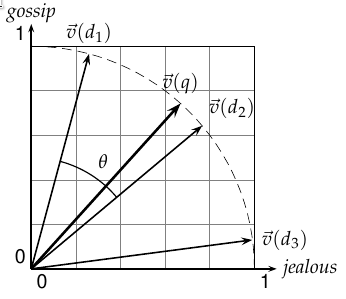
\includegraphics[scale = .5]{./images/ejemplosim.png}
\end{SCfigure}

Para calcular la similitud hacemos
$
    sim_{d_j, q} = cos{\theta}=\frac{d_j*q}{||d_j||||q||} = \frac{\sum_{n = 1}^{N} w_{i,j}w_{i,q} }
    { \sqrt{\sum_{n = 1}^{N} w_{i,j}^{2} } \sqrt{\sum_{n = 1}^{N} w_{i,q}^{2} }}
$

Con esto se tiene una ordenación por relevancia(los que tengan mayor similitud) de 
de los documentos respecto a la query .

\textbf{Implementación realizada en Python para el cálculo de la similitud}

\begin{python}
    def sim(self, v1: List[float], v2: List[float]) -> float:
        dotproduct = 0
        for i in range(len(v1)):
            dotproduct += v1[i]*v2[i]

        norm1 = 0
        for i in v1:
            norm1 += i*i
        norm1 = math.sqrt(norm1)

        norm2 = 0
        for i in v2:
            norm2 += i*i
        norm2 = math.sqrt(norm2)

        return dotproduct/(norm1*norm2)
    ....
\end{python}


Se puede establecer un umbral de similitud y quedarnos solamente con los documentos que son mayores 
que ese umbral.

\subsection {Razones por la que se escogió este modelo como el modelo principal del sistema:}
\noindent
$\bullet$
Este modelo es bastante sencillo de implementar y ofrece notables mejoras respecto al booleano.\\
\noindent
$\bullet$
La estrategia de coincidencia parcial permite la recuperación de documentos que se aproximen a los 
requerimientos de la consulta. \\
\noindent
$\bullet$
El esquema de ponderación tf-idf para los documentos mejora el 
rendimiento de la recuperación. \\
\noindent
$\bullet$
La fórmula del coseno ordena los documentos 
de acuerdo al grado de similitud con la consulta. 

\subsection {Limitaciones que tenemos al usar este modelo:}
$\bullet$
Uno de los problemas que tiene es la sensibilidad semántica; los documentos con un contexto similar 
pero con un vocabulario de términos diferente no se asociarán, lo que resultará en una coincidencia 
negativa falsa.\\
\noindent
$\bullet$
Teoricamente asume que los términos son estáticamente independientes\\
\noindent
$\bullet$
El orden en que los términos aparecen en el documento se pierde en la representación en el espacio vectorial

\subsection{Modelo Fuzzy:}
Se implementó como modelo secundario para tener la opción de elegir si se quería probar con el mismo. 

El modelo fuzzy es una extensión del modelo booleano. En este modelo cada término de la query es 
definido mediante un conjunto difuso y cada documento tiene un grado de pertenencia a dicho 
conjunto(valor entre 0 y 1). La idea básica es expandir el conjunto de términos de índice 
en la consulta con términos relacionados, de modo que la consulta del usuario pueda recuperar 
documentos relevantes adicionales. Se puede usar un thesaurus para modelar el problema de recuperación 
de información en términos de conjuntos difusos. Un thesaurus puede ser construido definiendo una 
matriz de correlación término a término cuyas filas y columnas están asociada a los términos  de la
colección de documentos. En dicha matriz, un factor de correlación normalizado $c_{i,l}$ entre 
dos términos $k_{i}$ y $k_{l}$ se define de la siguiente forma:\\

$
    c_{i,l} =  \frac{n_{i,l}}{n_i+n_l-n_{i,l}}
$
\\\\
\noindent
Donde $n_i$ es el número de documentos que contienen al término $k_i$, $n_l$ el número de documentos
que continen al término $k_l$, $n_{i,l}$ el  número de documentos que contienen a ambos términos \\
Podemos usar la matriz de correlación para definir un conjunto difuso asociado a cada término $k_i$.
En este conjunto difuso, un documento $d_j$ tiene un grado de pertenencia(grade of membership) $\mu_{i,j}$
que se define como:\\\\
$
\mu_{i,j} = 1 - \prod_{k_ln \in d_j}^{}  (1-c_{i,l}) 
$
\\\\
\noindent
Un documento $d_j$ pertenece al conjunto difuso asociado al término $k_i$ si sus  términos están relacionados 
con $k_i$. Siempre que haya un término $k_l$ de $d_j$ que esté fuertemente relacionado($c_{i,l}\sim 1$), 
entonces $\mu_{i,j} \sim 1$ y el término $k_i$ es un buen fuzzy index para el documento $d_j$. En el caso 
que todos los documemntos de $d_j$ estén pobremente relacionados con $k_i$, $k_i$ no es un buen fuzzy 
index para $d_j$($\mu_{i,j}\sim 0 $).\\\\ 

La similitud entre un documento $d_j$ y la query q se se define:

$
    sim(q,d_j) = 1 - \prod_{i=1}^{N} (1 - \mu_{k_i,d_j})
$

Donde N es la cantidad de términos de la query.

Entonces te puedes quedar con los documentos ordenados por ranking de relevancia 
respecto a la query.

Para la implementación de este modelo se definió una clase Fuzzy
\begin{python}
class Fuzzy:
def __init__(self, corpus_term, documents, compute_fuzzy_data_required: bool = False):
    self.corpus_terms: List['str'] = corpus_term 
    self.documents: List['Doc'] = documents
    self.correlation_matrix = {}
    if compute_fuzzy_data_required:
        self.compute_fuzzy_data()
    else:
        self.deg_memb_matrix = unpick_pickle_file('./preprocessed/deg_memb_matrix.pickle')
    ...
\end{python}

Recibe los términos del vocabulario y los documentos asi como el parámetro $compute\_fuzzy\_data\_required$
que indic si es necesario hacer el preprocesado de calcular la matriz de grado pertenencia o se 
puede cargar desde un file previamente salvado \textbf{.pickle}\\\\
\noindent
\textbf{Implementación hecha en Python para el c\'alculo de la matriz de correlación:}
\begin{python}
def correlation_factor(self, ki: str, kl: str):
    if (ki,kl) in self.correlation_matrix:
        return self.correlation_matrix[(ki, kl)]
    if (kl, ki) in self.correlation_matrix:
        return self.correlation_matrix[(kl, ki)]
    n_i = 0  
    n_l = 0
    n_i_l = 0 
    for doc in self.documents:
        if ki in doc.terms:
            n_i+=1
        if kl in doc.terms:
            n_l+=1
        if ki in doc.terms and kl in doc.terms:
            n_i_l +=1
    result = n_i_l/(n_i + n_l - n_i_l) # ci,l
    self.correlation_matrix[(ki, kl)] = result
    return result
...
\end{python}
\textbf{Implementación hecha en Python para el c\'alculo del grado de pertenencia 
de un documento dj al conjunto difuso de un término ki:}\\
\begin{python}
    def degree_of_membership(self, ki, dj): 
        if (ki, dj) in self.deg_memb_matrix:
            return self.deg_memb_matrix[(ki, dj)]
        result = 1
        for term in self.documents[dj].terms:
            result *= 1- self.correlation_factor(ki, term)
        result = 1 - result
        return result
    ...
\end{python}

\noindent
\textbf{Implementación hecha en Python para el cálculo de la similitud 
entre la query y un documento:}\\

\begin{python}
    def sim(self, q, dj): 
        result = 1

        for t in q:
            result *= 1 - self.deg_memb_matrix[(t, dj)]

        result = 1- result
        return result
    ...
\end{python}


Para obtener los documentos más relevantes se va por cada documento se calcula 
la similitud de cada uno con la query como se explicó anteriormente y al 
final se hace un ranking por relevancia bastante similar a como es con el vectorial.
También se puede considerar un umbral de similitud y quedarte solamente con los resultados
por encima de dicho umbral.


\section{Obtención de resultados de la búsqueda:}

Para buscar los resultados cada clase que representa los 2 modelos empleados tiene un 
método que se llama $get\_search\_results$ que es al que se llama una vez obtenido el texto 
de lo que escribió el usuario en la componente gráfica que tiene para escribir texto.

\begin{python}
def get_search_results(self,*, query: str,
    filters: List[str],
    top10: bool = False):
    ....
\end{python}

Según lo que se le pase en el parámetroo filters devolvera solo los documentos que cumplan 
con el  o los tipos de documentos  especificados, si se le pasa top10 en True solo 
devuelve los 10 primeros resultados del ranking.




\section{Interfaz gráfica y como puede buscar las consultas el usuario:}

La interfaz gráfica se desarrollócon \textbf{streamlit} una biblioteca bastante cómoda para 
crear aplicaciones de interfaz web desde Python. En el file $UI\_streamlit.py$ 
está el código de la parte gráfico del sistema de recuperación de información 
desarrollado.

\begin{SCfigure}[0.5]
    \caption{Interfaz para hacer búsquedas}
    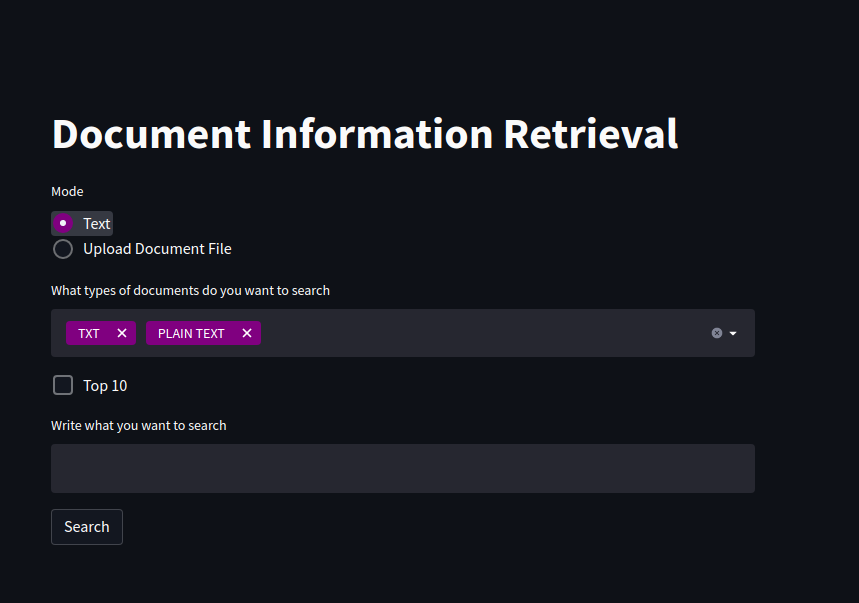
\includegraphics[scale = .28]{./images/ui_tex_search.png}
    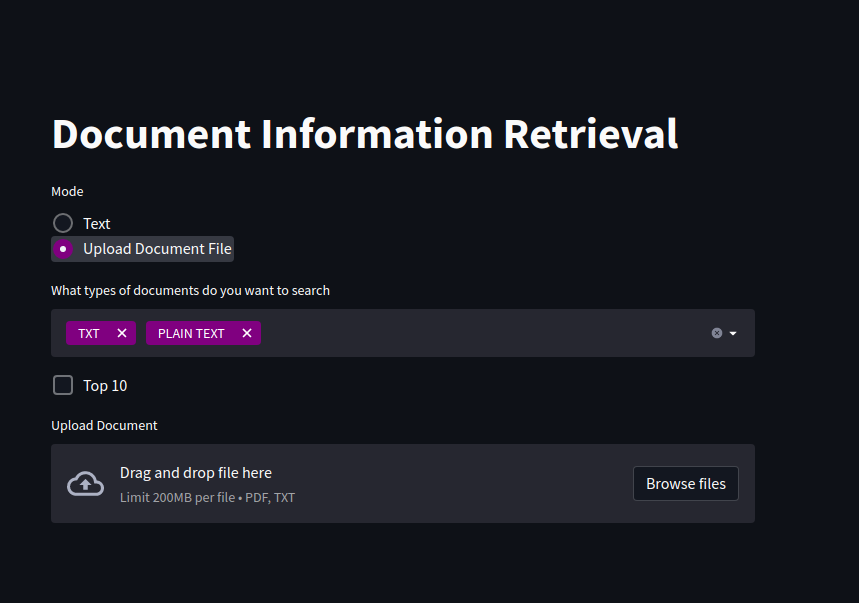
\includegraphics[scale = .28]{./images/ui_uploadsearch.png}
\end{SCfigure}

\noindent
Como se puede observar se pueden hacer búsquedas tanto escribiendo directamente 
lo que se quiere buscar en la barra de búsqueda así como arrastrando o subiendo 
un file de documento en los posibles formatos aceptados(PDF y TXT).


\begin{SCfigure}[0.5]
    \caption{Si no se encuentra ningún resultado a la búsqueda}
    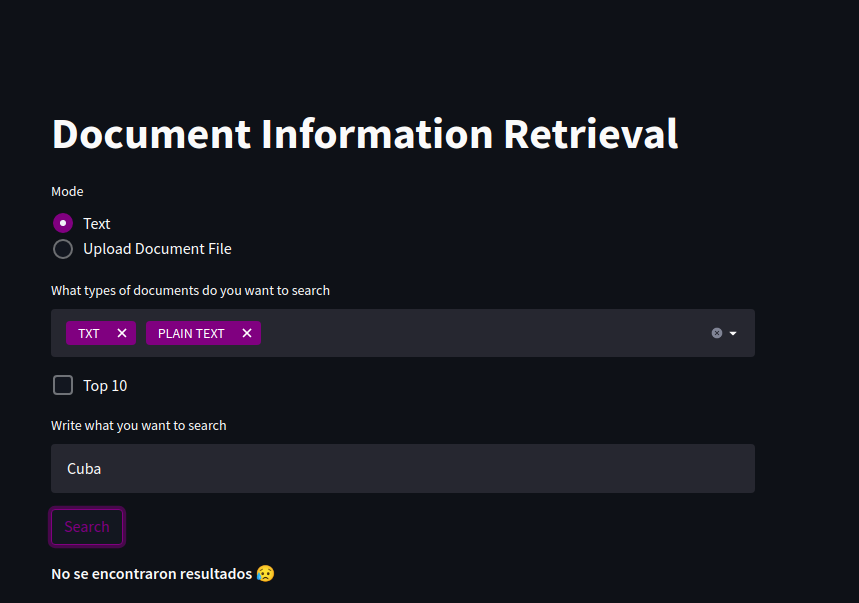
\includegraphics[scale = .28]{./images/ui_notfouund.png}
\end{SCfigure}

En caso que se encuentren resultados a la búsqueda del usuario 
se visualizará para cada documento el nombre del documento 
una imagen que identifica el tipo de documento que es y un botón
para descargar el archivo si se quiere. Además se pueden filtrar 
los resultados por solo un tipo (PDF, txt, text plane) o poniendo 
que solo te quieres quedar con los 10 primeros resultados (Top10).


\begin{SCfigure}[0.5]
    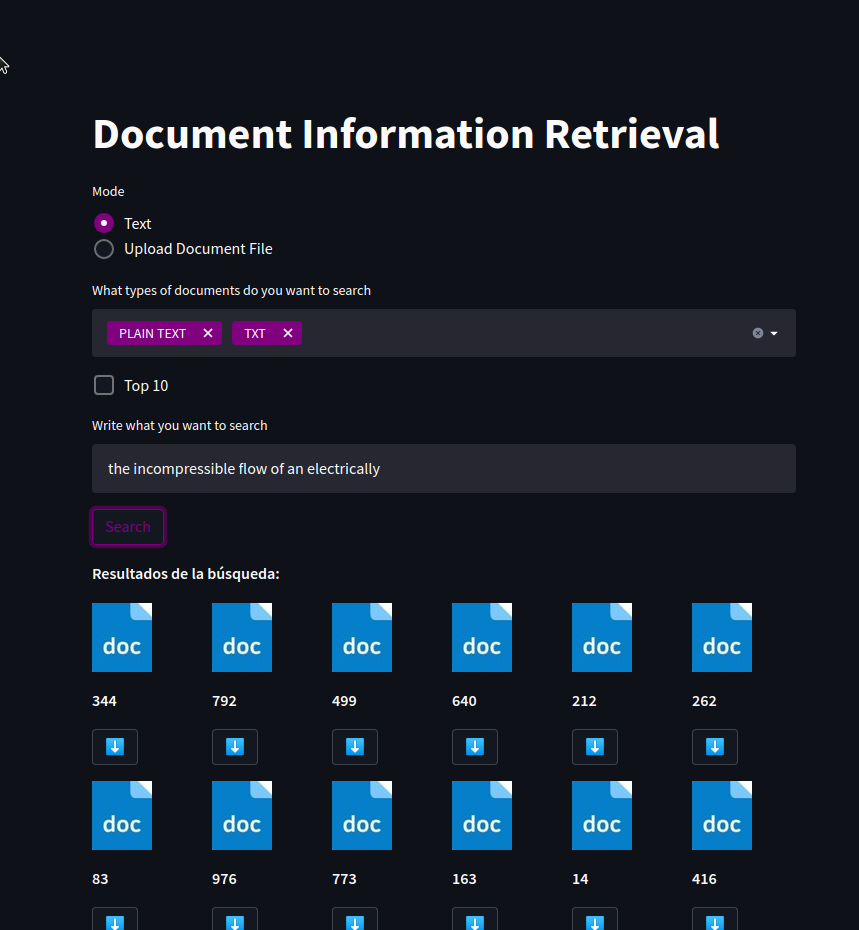
\includegraphics[scale = .28]{./images/ui_search_result.png}
    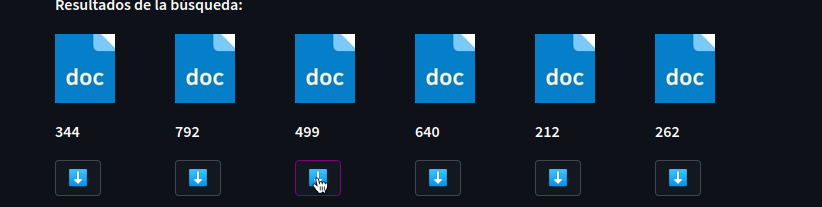
\includegraphics[scale = .28]{./images/ui_tex_download.png}
    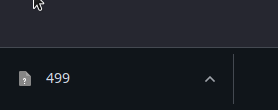
\includegraphics[scale = .28]{./images/file_downloaded.png}
\end{SCfigure}

\begin{SCfigure}[0.5]
    \caption{Solo Top10}
    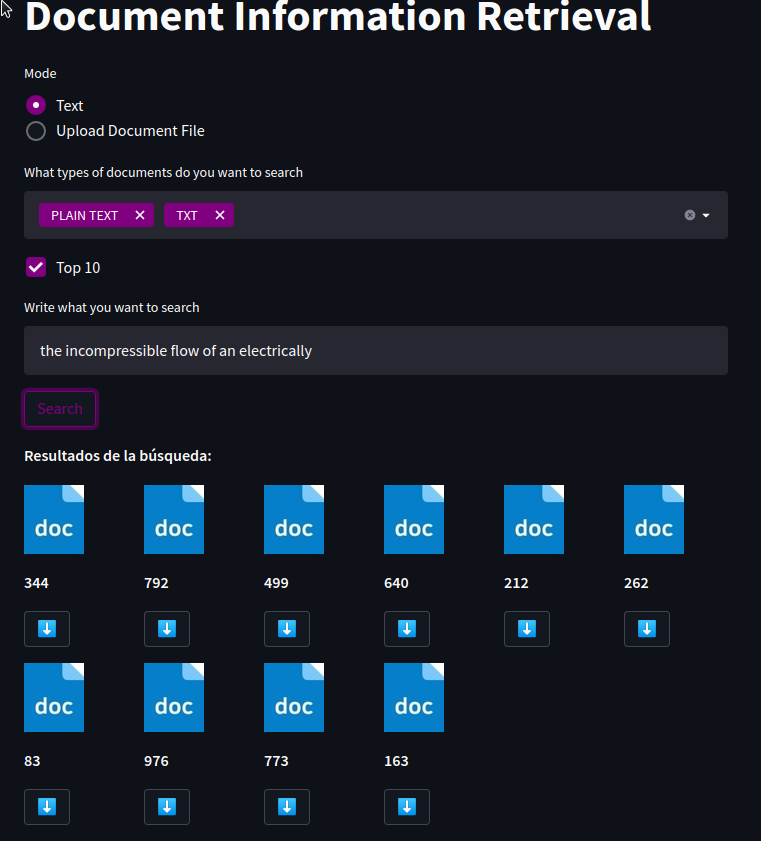
\includegraphics[scale = .28]{./images/top_10_sear.png}
    
\includegraphics[scale = .28]{./images/top_10.png}
    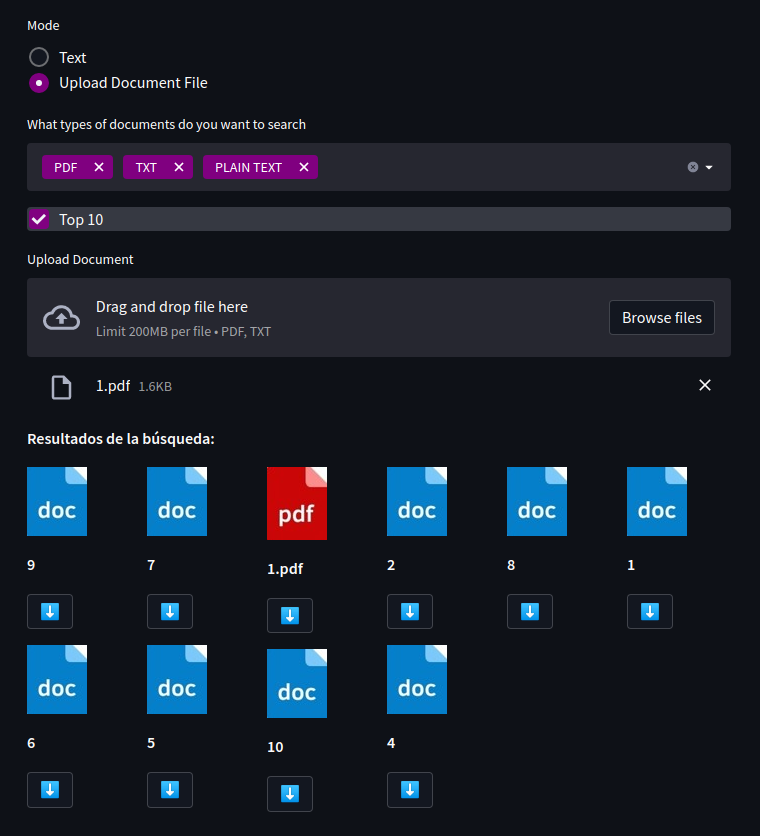
\includegraphics[scale = .28]{./images/top10_2.png}
\end{SCfigure}


\begin{SCfigure}[0.5]
    \caption{Solo PDF}
    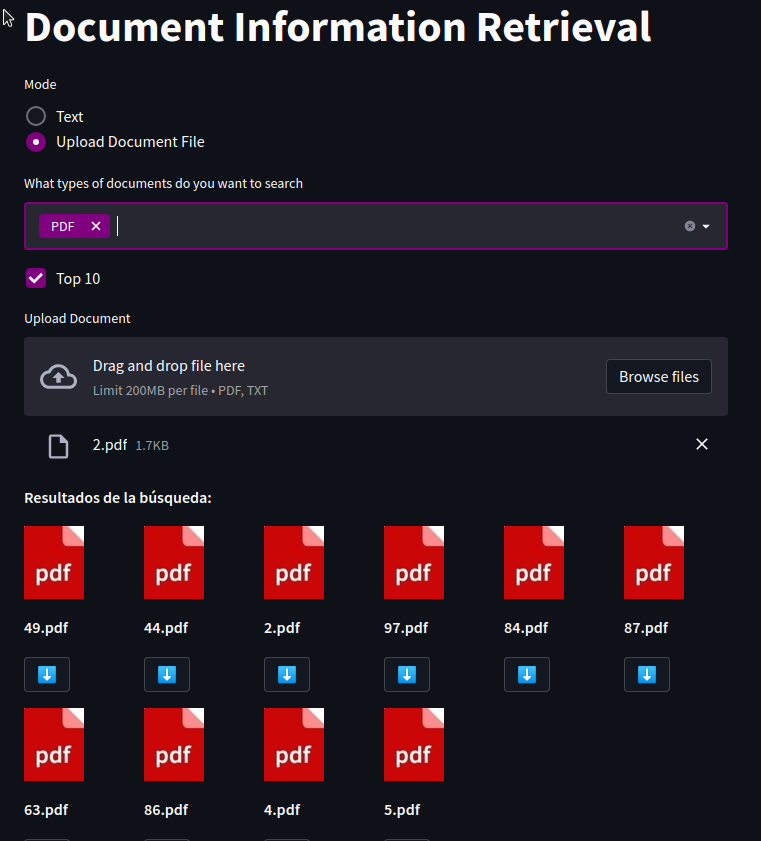
\includegraphics[scale = .28]{./images/only_pdf.png}
\end{SCfigure}

\begin{SCfigure}[0.5]
    \caption{Solo txt}
    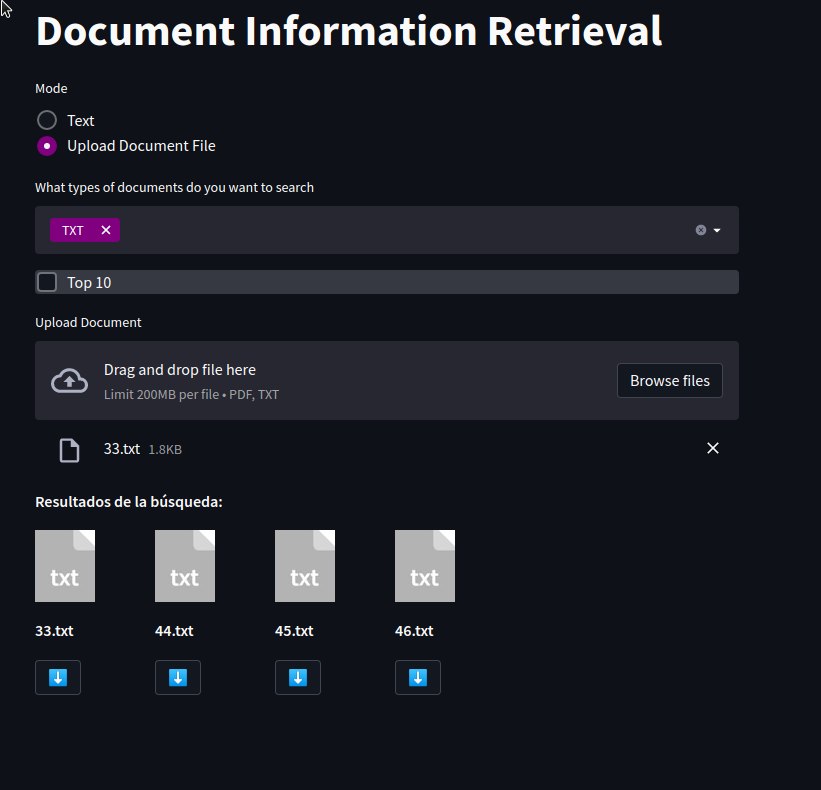
\includegraphics[scale = .28]{./images/onlytxt.png}
\end{SCfigure}

\chapter*{Evaluación del Sistema:}
\addcontentsline{toc}{chapter}{Evaluación del Sistema}

La evaluación del sistema la hicimos usando el modelo principal (el vectorial) pues el cálculo 
de la matriz de correlación término a término y el grado de pertenencia del fuzzu era muy 
costoso de computar con los corpus que probamos.\\

\noindent
Para la evaluación del sistema utilizamos tres colecciones de prueba:\\\\

\noindent
$\bullet$ \textbf{Cranfield} que tiene 1400 documentos y 225 querys de prueba\\
$\bullet$ \textbf{Medline} una colección de artículos de una revista médica que contiene 1033 documentos y 30 querys de prueba\\ 
$\bullet$ \textbf{Time} una colección de artículos de la revista Time que contiene 423 documentos y 83 querys de pruba.\\

\noindent
Las pruebas se realizaron con un umbral $> 0$.\\
Las medidas de evaluación que se emplearon fueron la precisión, el recobrado(recall), la medida F1,
el fallout, la r-precisión para 10 y el r-fallout para 10.\\
Para cada colección de prueba se calculó el promedio de las medidas menciandas con todas las querys
Los resultados obtenidos fuerons los siguientes:\\\

\begin{SCfigure}[0.5]
    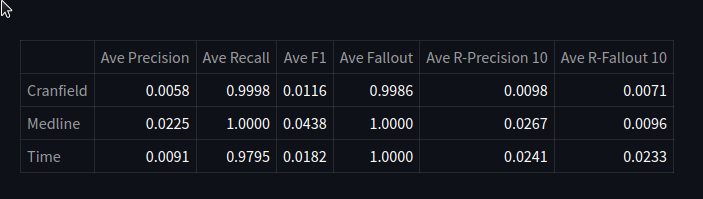
\includegraphics[scale = .7]{./images/umbrarl_ma0.png}
\end{SCfigure}


Como se puede observar en los resultados la precisión fue bastante baja pero tuvo un recobrado bastante
alto. Por tanto a pesar de que se recuperaron muchos documentos irrelevantes, la mayoría de los documentos 
relevantes fueron recuperados. Como el fallout da bastante elevado se recuperó un gran número de documentos 
irrelevantes.



\chapter*{Algunos consideraciones para mejorar el sistema implementado:}
\addcontentsline{toc}{chapter}{Algunos consideraciones para mejorar el sistema implementado}
Se puede agregar más formatos parar procesar desde documentos word, powerpoint,
html,epub  asi como procesar imágenes que contengas texto. Se podría tener coincidencias 
de palabras  que fuesen sinónimos y hacer tener búsquedas más cercanas a lo que desee el usuario.
Además agregar nuevas funcionalidades a la interfaz de usuario como mostrar un preview del documento 
sin tener que descargarlo o tener autocompletamiento en la búsqueda por texto matcheando con los 
términos que están en el vocabulario y se acerquen a lo que el usuario está buscando. También se 
podríá agregar alguna forma de analizar el contexto de lo que se habla en el documento o asignar 
tags para tenerlos separados por temáticas por ejemplo.
\newpage

\chapter*{}
\addcontentsline{toc}{chapter}{References}
\begin{thebibliography}{}
    %
    \bibitem[1]{2clar:eke}
    Cristopher D. Manning, Prabhakar Raghavan, Hinrich Schutze (2009).
    An introduction to Information Retrieval.
    
    \bibitem[2]{2clar:eke:2}
    Baeza-Yates(2002).
    Modern Information Retrieval 

   
    \bibitem[3]{2rab}
    Unknown Author.
    Documentación de Streamlit.Streamlit.\url{https://docs.streamlit.io/}.
    \bibitem[4]{2rab}
    Unknown Author.
    Documentación de NLTK\url{ https://www.nltk.org/}.
    
\end{thebibliography}



\end{document}